\documentclass{article}
\usepackage{amsmath}
\usepackage{xcolor}
\usepackage{amsthm}
\usepackage{graphicx}
\usepackage{unicode-math}
\usepackage{hyperref}
\usepackage{datetime}
\usepackage{todonotes}
\usepackage{bbm}

% inline comments
% you could use \listoftodos to print an overview
\newcommand{\inline}[1]{ {\color{blue}{#1}}\addcontentsline{tdo}{todo}{#1}}
\newcommand{\comment}[1]{{\color{blue}\noindent{#1}\\}\addcontentsline{tdo}{todo}{#1}}
% use this one to disable
%\newcommand{\inline}[1]{\ignorespaces}


\newdateformat{monthyeardate}{\monthname[\THEMONTH] \THEYEAR}

\newcommand{\newmarkedtheorem}[1]{%
  \newenvironment{#1}
    {\pushQED{\qed}\csname inner@#1\endcsname}
    {\popQED\csname endinner@#1\endcsname}%
  \newtheorem{inner@#1}%
}

\theoremstyle{definition}
%\newtheorem{eg}{Example}[section]
\newmarkedtheorem{eg}{Example}[section]
\newtheorem{observation}{Observation}[section]
\theoremstyle{plain}
\newtheorem{define}{Definition}[section]
\newtheorem{proposition}{Proposition}[section]
\newtheorem{theorem}{Theorem}[section]
\newtheorem{assump}{Assumption}[section]
\newtheorem{remark}{Remark}[section]


\title{Single Intersection Scheduling with Deep Q-Learning}
\author{Jeroen van Riel}
\date{\monthyeardate\today}

\begin{document}

\maketitle

\section{Introduction}

Recall our definition of the Single Interesection Scheduling Problem. We saw
that it can be concisely formulated as a Mixed-Integer Linear Program.
Therefore, one direct solution approach is to apply standard software for
solving this class of problems. We will use the commercial Gurobi solver.
Alternatively, we will show how the problem can be formulated in terms of
\textit{dispatching} jobs. We will argue that this formulation allows us to
tackle the problem with reinforcement learning techniques and compare the
performance of these methods to that of the exact procedure.

\section{Environment}

We are interested in whether we can learn a procedure to generate good
schedules. To start with, we propose to focus on dispatching procedures, which
means that the schedule is constructed by inserting jobs one by one. Therefore,
we will define this procedure in terms of a Markov Decision Process (MDP).

% basic setup
Assume we have a single intersection with $K$ lanes. Because this corresponds
with a single machine in the machine scheduling context, we will use the first
index to refer to the lane, so we use $r_{ij}$ and $p_{ij}$ to denote the
release date and processing time, respectively, of the $j$th platoon of vehicles
on lane $i$. Note that it is not necessary to specify the number of vehicles of
a platoon, because of the Platoon Preservation Theorem. Instead, we only
consider the total processing time.

% arrival processes
Let $i \in \{0, \dots, K - 1\}$ be an arbitrary lane and let $n_{i}$ denote the
(possibly infinite) number of total arrivals to this lane. The release dates and
processing times can be considered part of the specification of the MDP, which
means that $(r_{ij})_{j=1}^{n_{i}}$ and $(p_{ij})_{j=1}^{n_{i}}$ are fixed. In
the following experiments, we assume that the arrival process is as follows.
% processing times
We assume the processing times are integers distributed as $p_{ij} \sim \text{Uni}[L, H]$.
{\color{gray}
The processing times are distributed as $p_{ij} \sim \text{Geom}(\theta)$ such
that $P(p_{ij} = n) = (1-\theta)^{n-1}\theta$, so it is the required number of
Bernoulli trials before the first success, where $\theta$ is the success
probability.
}
% release dates
We define interarrival times $X_{ij} \sim \text{Exp}(\lambda)$, parameterized
such that $\mathbb{E}[X_{ij}] = \lambda$. The release dates are given by
\begin{align}
r_{ij} = \sum_{l=1}^{j-1} p_{il} + \sum_{l=1}^{j} X_{il} .
\end{align}

% actions
In a dispatching approach, platoons are assigned to a timeslot one by one.
Because of the precedence constraints between platoons on the same lane, this is
equivalent to deciding in which order to serve the lanes. Therefore, the action
$a$ of the scheduler is to decide whether to keep serving the current lane
($a = 0$), or to serve the next lane ($a = 1$).
% state space
At step $t$, let $c^{(t)}$ denote the lane that was last served and let
$m_{i}^{(t)}$ denote the number of scheduled platoons from lane $i$. Let
$T^{(t)}$ denote the completion time of the last scheduled platoon at step $t$,
so before any platoons are scheduled, we have $T^{(0)} = 0$. The state at step
$t$ can then simply be written as
\begin{align}
   s^{(t)} = (c^{(t)}, T^{(t)}, m_{1}^{(t)}, \dots, m_{K}^{(t)} ) \in \{1, \dots, K\} \times \mathbb{R} \times \mathbb{N}^{K} .
\end{align}
% compute the starting times from the state
Note that we do not consider the starting times $y_{ij}$ to be explicitly part
of the state, because only completion time $T^{(t)}$ of the last scheduled
platoon is necessary for the state to be Markovian.

% transitions
Furthermore, the state transitions are very simple. Whenever the same lane is
served, $a^{(t)}=0$, we have $c^{(t+1)} = c^{(t)}$, when serving the next lane,
$a^{(t)}=1$, we have $c^{(t+1)} = c^{(t)} + 1 \mod K$. The completion time
$T^{(t+1)}$ is calculated as follows. To simplify notation, let
$i^{(t)} = c^{(t+1)}$ and $j^{(t)} = m_{i^{(t)}}^{(t)} + 1$, then
\begin{align}
  T^{(t+1)} = T^{(t)} + s a^{(t)} + p_{i^{(t)}j^{(t)}} ,
\end{align}
where $s$ is the switch-over time. Observe that the pair $(i^{(t)}, j^{(t)})$
identifies the platoon that is scheduled in the transition from $t$ to $t+1$
with starting time given by
\begin{align}
  y_{i^{(t)}j^{(t)}} = T^{(t)} + s a^{(t)} .
\end{align}
For the remaining part of the state, with $i \in \{0, \dots, K\}$, we always
have
\begin{align}
  m_{i}^{(t+1)} = m_{i}^{(t)} + \mathbb{1}\{ i = i^{(t)} \} .
\end{align}

% reward
Recall that we defined the objective for optimal schedules as minimizing the
total delay for platoons. When assuming $n_{i} < \infty$ for all lanes $i$, we
could decide to only define episodic reward according to total delay in the
complete schedule. However, to deal with possibly infinite episodes and to
provide the scheduler with earlier reward signals, we define the reward to be
\begin{align}
  r^{(t)} = (y_{i^{(t)}j^{(t)}} - r_{i^{(t)}j^{(t)}}) \cdot p_{i^{(t)}j^{(t)}} .
\end{align}

% partial observability: horizon
As we indicated above, the exact arrivals $\{(p_{ij}, l_{ij})_{j=1}^{\infty}\}_{i=1}^{K}$ can
be considered a fixed part of the specification of a particular instance of the
MDP. Therefore, we regard it as a constant part of the state. When the scheduler
has no access to these arrivals in any way, it is not very interesting to solve
the MDP. Therefore, we should further specify what information is available to
the scheduler. By defining the exact \textit{observations} that become available
to the scheduler, we obtain a Partially Observable Markov Decision Process
(POMDP).

% observations
We assume that the scheduler does not know about all arrivals upfront, but sees
a certain number $h_{i}^{(t)}$ of next arrivals at lane $i$. Thefore, the
visible \textit{horizon} of lane $i$ at step $t$ consists of the release dates
and processing times
\begin{align}
  \mathcal{H}_{i}^{(t)} = \{ (p_{ij}, l_{ij}) : j \in \{ m_{i}^{(t)}, m_{i}^{(t)} + 1, \dots, m_{i}^{(t)} + h_{i}^{(t)} \} \} .
\end{align}
Therefore, the observation at step $t$ is deterministic and given by
\begin{align}
  o^{(t)} = \{ \mathcal{H}_{i}^{(t)} \}_{i=1}^{K} .
\end{align}
In general, the length $h_{i}^{(t)}$ of the horizon may depend on the arrival
times. This would be the case when we want to model a fixed look-ahead time
$t_{a}$. However, in what follows, we will assume that $h_{i}^{(t)} = h$ for
some fixed $h$. This makes the implementation simpler, because the vector that
encodes the horizon has fixed dimensions in this case, so we do not have to
implement some sort of \textit{masking}.



\section{Deep Q-Learning}

Let the \textit{total discounted return} from step $t$ be defined as
\begin{align}
  G_{t} = \sum_{k=0}^{\infty} \gamma^{k} R_{t+k+1} ,
\end{align}
where $\gamma$ is the \textit{discount factor}. The state-action value
$q_{\pi}(s, a)$ is defined as the expected total discounted return by taking
action $a$ in state $s$ and following $\pi$ afterwards, so we have
\begin{align}
  q_\pi(s,a) = \mathbb{E}_{\pi}[ G_{t} | S_{t} = s, A_{t} = a ] ,
\end{align}
for all $s \in \mathcal{S}$ and $a \in \mathcal{A}$. These values are also
refered to as \textit{q-values}. It turns out that all optimal policies share
the same q-values, so the optimal state-action value function can be defined as
\begin{align}
  q_{*}(s, a) = \max_{\pi} q_{\pi}(s, a) .
\end{align}
It can be shown that
\begin{align}
  q_{*}(s, a) &= \mathbb{E} \left[ R_{t+1} + \gamma \max_{a'} q_{*}(S_{t+1}, a') \right] ,
\end{align}
which is known as the \textit{Bellman equation}.

The main goal of Q-learning is to estimate the optimal q-values. This is done using the following \textit{temporal difference update}
\begin{align}
  \hat{q}(s_{t}, a_{t}) \leftarrow  \hat{q}(s_{t}, a_{t}) + \alpha [ r_{t+1} + \gamma \max_{a} \hat{q}(s_{t+1}, a) - \hat{q}(s_{t}, a_{t}) ] .
\end{align}
This method is an \textit{off-policy} method, because it can be shown that
$\hat{q}$ will converge to $q_{*}$ regardless of the policy $\pi$ that is being
followed, as long as all states are visited infidelity often.

\subsection{Function approximation}


\subsection{Experience replay}


\section{Experiments}

Assume we have two lanes, with fixed switch-over time $s=2$ and a fixed number
of arrivals $n=30$ for each lane. We assume that $p_{ij} \sim \text{Uni}[1, 3]$.
Consider four scenarios with
$\lambda_{1} = 2, \lambda_{2} = 3, \lambda_{3} = 4, \lambda_{4} = 5$.

We ue the commercial Gurobi solver to obtain an estimate for the optimal
expected objective. More precisely, we estimate
\begin{align}
\mathbb{E}\left[ \sum_{j} C_{j} \right] ,
\end{align}
where the expectation is given over the distribution of the arrival process
\begin{align}
\{(p_{ij}, l_{ij})_{j=1}^{\infty}\}_{i=1}^{K}
\end{align}
as defined above. To estimate this quantity, we solve \textbf{100} randomly generated
instances with an optimality gap of $g = 0.1$.

For the DQN, we use a fixed horizon of $h = 10$. The smoothed return obtained by
a \textbf{single run} of the DQN algorithm for each scenario is shown in
Figure~\ref{fig:dqn-learning-rates}.

\begin{table}
  \centering
\begin{tabular}{|c|r|r|}
  $\lambda$ & exact ($g=0.1$) & dqn ($h=10$) \\
  \cline{1-3}
  2 & -705 & -1012 \\
  3 & -445 & -375 \\
  4 & -258 & -251 \\
  5 & -185 & -201
\end{tabular}
\caption{Episodic reward (rounded to integers) for each of the four scenarios
  for both methods. The results for the exact approach are averaged over 100
  randomly generated instances. The results for the DQN method are obtained from
  a single run (consisting of multiple episodes).}
\end{table}

\begin{figure}
  \centering
  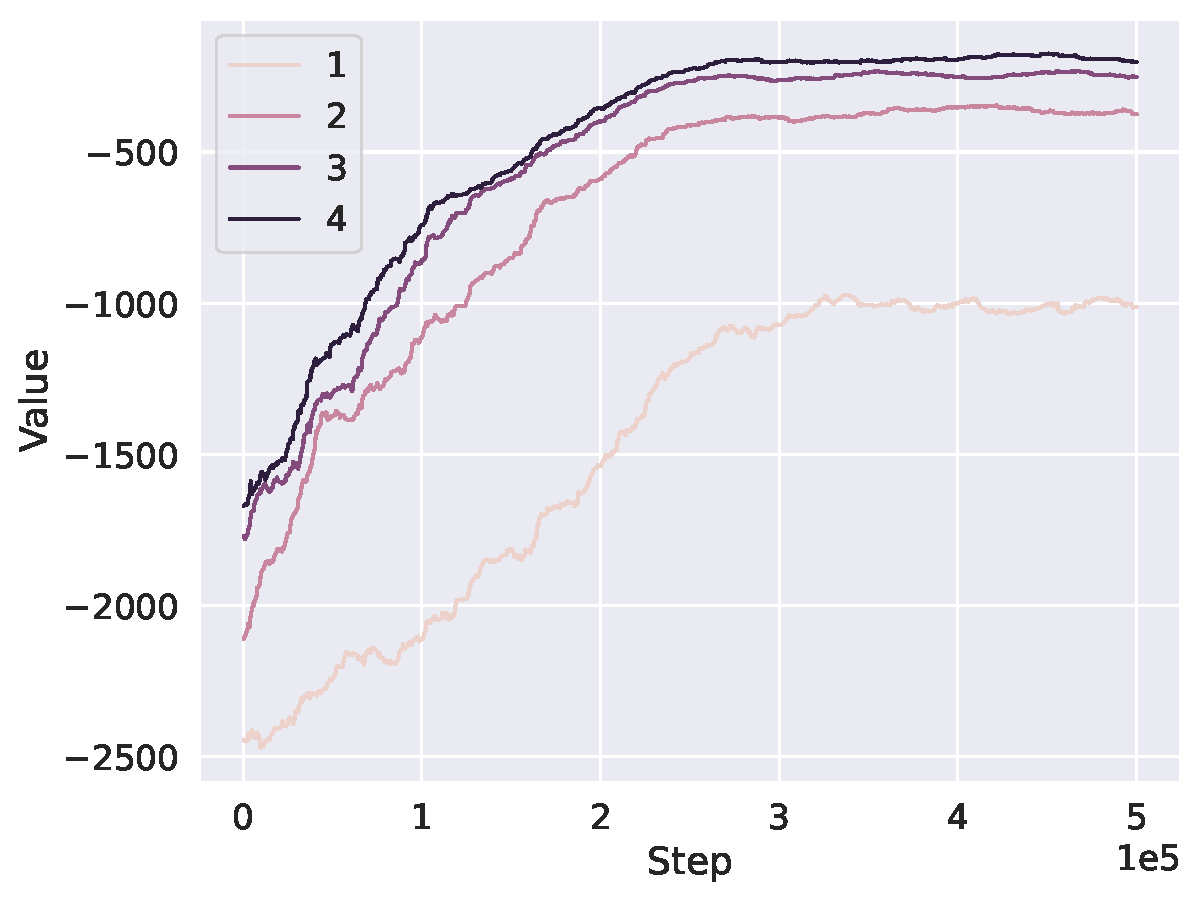
\includegraphics[width=0.9\textwidth]{../single-intersection/comparison.pdf}
  \label{fig:dqn-learning-rates}
\end{figure}

% \bibliography{references}
% \bibliographystyle{ieeetr}

\end{document}
